% Figure from MATH 493 notes, section 50 (lecture 10/30, Jordan-Hoelder).
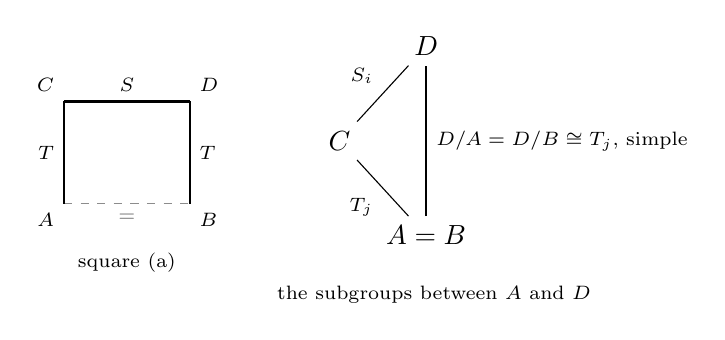
\begin{tikzpicture}[x=1cm, y=1cm]
\draw[black, thick] (0, 1.3) -- (1.6, 1.3);
\node[above, black, font=\scriptsize] at (0.80,1.30) {$S$};
\draw[black!45, dashed] (0, 0) -- (1.6, 0);
\node[below, black!55, font=\scriptsize] at (0.80,0.00) {$=$};
\draw[black, thick] (0, 0) -- (0, 1.3);
\node[left, black, font=\scriptsize] at (0.00,0.65) {$T$};
\draw[black, thick] (1.6, 0) -- (1.6, 1.3);
\node[right, black, font=\scriptsize] at (1.60,0.65) {$T$};
\node[below left, font=\scriptsize] at (0,0) {$A$}; \node[below right, font=\scriptsize] at (1.6,0) {$B$};
\node[above left, font=\scriptsize] at (0,1.3) {$C$}; \node[above right, font=\scriptsize] at (1.6,1.3) {$D$};
\node[font=\scriptsize] at (0.8,-0.75) {square (a)};
\begin{scope}[shift={(4.6,-0.4)}]
\node (D) at (0,2.4) {$D$};
\node (C) at (-1.1,1.2) {$C$};
\node (A) at (0,0) {$A = B$};
\draw (A) -- node[below left, font=\scriptsize] {$T_j$} (C);
\draw (C) -- node[above left, font=\scriptsize] {$S_i$} (D);
\draw[thick] (A) -- node[right, font=\scriptsize] {$D/A = D/B \cong T_j$, simple} (D);
\node[font=\scriptsize, align=center] at (0.1,-0.75) {the subgroups between $A$ and $D$};
\end{scope}
\end{tikzpicture}
